\section{Implementation}

\subsection{Methodology}

This section describes the implemented end-to-end workflow: data ingestion, data cleaning, canonical table construction, agreement analysis, supervised learning, weak supervision, pseudo-labeling, final model selection, reporting, and demo inference. The system is designed as an offline batch pipeline for harmful video detection, with a small API for local prediction after the model is trained.

\subsubsection{System Architecture}

The system follows a staged batch architecture. Raw labeled and unlabeled files are first ingested into a preservation layer. They are then normalized into a common schema, consolidated into a modeling table, split into training, validation, and test sets, and finally used to train and compare multiple model variants. The selected model is exposed through a local prediction API.

\begin{figure}[H]
\centering
\resizebox{0.98\textwidth}{!}{
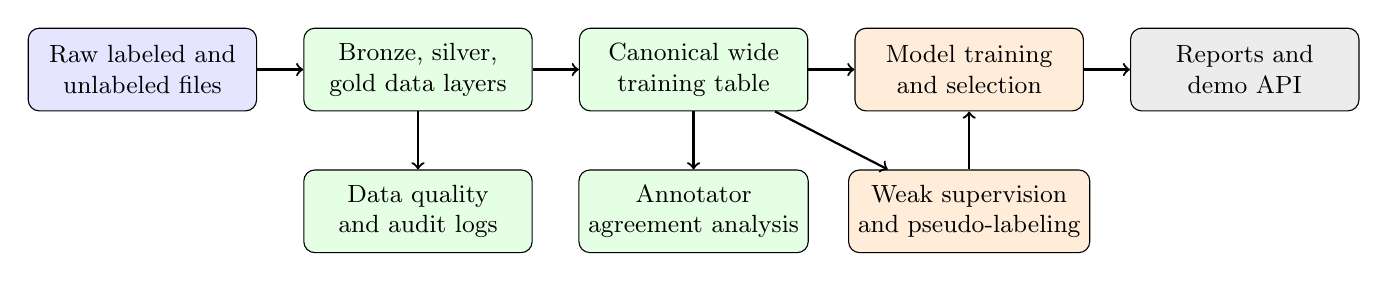
\begin{tikzpicture}[
    box/.style={draw, rounded corners, align=center, minimum width=2.9cm, minimum height=1.05cm, font=\small},
    data/.style={box, fill=blue!10},
    process/.style={box, fill=green!10},
    model/.style={box, fill=orange!15},
    output/.style={box, fill=gray!15},
    arrow/.style={->, thick}
]
\node[data] at (0,1.8) (raw) {Raw labeled and\\unlabeled files};
\node[process] at (3.5,1.8) (lake) {Bronze, silver,\\gold data layers};
\node[process] at (7.0,1.8) (wide) {Canonical wide\\training table};
\node[model] at (10.5,1.8) (train) {Model training\\and selection};
\node[output] at (14.0,1.8) (api) {Reports and\\demo API};

\node[process] at (3.5,0.0) (audit) {Data quality\\and audit logs};
\node[process] at (7.0,0.0) (agreement) {Annotator\\agreement analysis};
\node[model] at (10.5,0.0) (pseudo) {Weak supervision\\and pseudo-labeling};

\draw[arrow] (raw) -- (lake);
\draw[arrow] (lake) -- (wide);
\draw[arrow] (wide) -- (train);
\draw[arrow] (train) -- (api);
\draw[arrow] (lake) -- (audit);
\draw[arrow] (wide) -- (agreement);
\draw[arrow] (wide) -- (pseudo);
\draw[arrow] (pseudo) -- (train);
\end{tikzpicture}
}
\caption{Implemented batch architecture for text-first harmful video detection.}
\label{fig:implementation-system-architecture}
\end{figure}

The architecture is intentionally modular. Data engineering is separated from modeling so that source cleanup, label normalization, and leakage checks can be verified before training. Model comparison is also separated from final API inference so that the deployed demo always uses the selected model rather than an arbitrary training run.

\subsubsection{Technology Stack}

The implementation uses Python for the main workflow, local PySpark for big-data-style pipeline orchestration and schema validation, pandas and spreadsheet readers for Excel ingestion, CSV parsing with NUL-byte cleanup for the unlabeled pool, Parquet for columnar storage, scikit-learn for text modeling, Matplotlib and Seaborn for reporting visuals, and FastAPI for the local prediction service.

The project also includes a containerized execution path. This is useful because local Spark execution can be sensitive to operating-system-specific Java and filesystem behavior. The containerized path provides a more reproducible Linux environment for running the batch pipeline and demo API.

\subsubsection{Data Sources}

The dataset contains multiple source groups. Domain expert labels are treated as the primary supervised ground truth. GPT-4-Turbo and crowdworker labels are treated as weak supervision sources. Agreement subsets are used to support robustness analysis, and the unlabeled pool is used for pseudo-labeling.

\begin{table}[H]
\centering
\small
\renewcommand{\arraystretch}{1.25}
\begin{tabularx}{\textwidth}{|>{\raggedright\arraybackslash}p{3.2cm}|>{\raggedright\arraybackslash}X|>{\raggedright\arraybackslash}p{3.2cm}|}
\hline
\textbf{Source group} & \textbf{Role in the project} & \textbf{Modeling use} \\
\hline
Domain expert harmful and harmless labels & Main human expert annotation source for binary harmful vs harmless detection. & Primary supervised ground truth. \\
\hline
GPT-4-Turbo harmful and harmless labels & Machine-generated annotations over overlapping and non-overlapping videos. & Weak supervision source. \\
\hline
Crowdworker harmful and harmless labels & Human crowd annotations with broader but noisier coverage. & Weak supervision source. \\
\hline
Agreement subsets & Videos with stronger agreement patterns across sources. & Secondary strict benchmark. \\
\hline
Unlabeled pool & Videos with text fields but no accepted expert, GPT, or crowdworker label. & Candidate pool for pseudo-labeling. \\
\hline
\end{tabularx}
\caption{Dataset source groups and their roles in the system.}
\label{tab:implementation-source-groups}
\end{table}

\subsubsection{Data Lake Construction}

The data pipeline uses bronze, silver, and gold layers. The bronze layer preserves raw source records and ingestion metadata. The silver layer normalizes all sources into a shared schema. The gold layer builds the canonical wide table, train/validation/test split, agreement summaries, and audit outputs.

\begin{figure}[H]
\centering
\resizebox{0.94\textwidth}{!}{
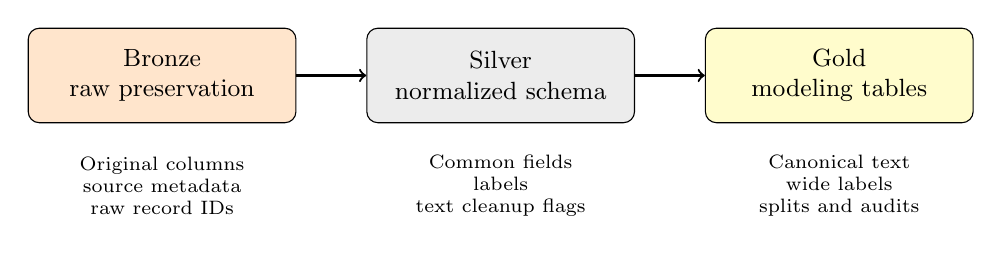
\begin{tikzpicture}[
    layer/.style={draw, rounded corners, align=center, minimum width=3.4cm, minimum height=1.2cm, font=\small},
    note/.style={align=center, font=\scriptsize},
    arrow/.style={->, thick}
]
\node[layer, fill=orange!20] at (0,0) (bronze) {Bronze\\raw preservation};
\node[layer, fill=gray!15] at (4.3,0) (silver) {Silver\\normalized schema};
\node[layer, fill=yellow!20] at (8.6,0) (gold) {Gold\\modeling tables};

\node[note] at (0,-1.4) {Original columns\\source metadata\\raw record IDs};
\node[note] at (4.3,-1.4) {Common fields\\labels\\text cleanup flags};
\node[note] at (8.6,-1.4) {Canonical text\\wide labels\\splits and audits};

\draw[arrow] (bronze) -- (silver);
\draw[arrow] (silver) -- (gold);
\end{tikzpicture}
}
\caption{Three-layer data organization used by the pipeline.}
\label{fig:implementation-data-layers}
\end{figure}

The silver schema includes the following main fields: video identifier, platform, source group, annotator source, binary label, raw harm labels, parsed harm-label array, title, description, transcript, published date, text-present flag, and ingestion issue flags. This shared schema makes it possible to join and compare labels from different sources without manually handling each file format during modeling.

\subsubsection{Data Cleaning and Audit Rules}

The data contains several source-specific quality issues. The pipeline handles column naming differences, misspelled description fields, padded blank spreadsheet rows, embedded NUL bytes in the unlabeled CSV, malformed CSV lines, and a duplicate crowdworker harmless source. Rows with missing video identifiers are dropped because they cannot be joined or split safely.

The most important cleaning rules are:

\begin{itemize}
    \item Normalize equivalent text columns such as title, description, transcript, and date even when source files use different capitalization or spelling.
    \item Remove embedded NUL bytes before parsing the unlabeled CSV.
    \item Skip malformed CSV lines and count them as ingestion issues.
    \item Exclude duplicate source files after detecting that they repeat an already ingested source.
    \item Drop records with missing video identifiers.
    \item Flag records with no usable title, description, or transcript.
\end{itemize}

The audit design is important because data cleaning changes the effective training set. Every dropped, merged, duplicated, or conflicted record should be explainable after the pipeline runs.

\subsubsection{Canonical Text and Wide Label Table}

Multiple rows may refer to the same video identifier because the same video can appear in several source files. The system builds one canonical wide row per video. The binary labels from domain experts, GPT-4-Turbo, and crowdworkers are stored side by side, while the text fields are selected by a deterministic canonical rule.

\begin{verbatim}
for each video_id and each text field:
    keep the longest non-empty normalized value
\end{verbatim}

This rule favors richer text when duplicated rows contain partial information. For example, if one source has only a title and another source has a longer transcript for the same video, the canonical row keeps the longer available transcript. The system also records which source supplied the selected canonical field, making the merge auditable.

The wide table contains:

\begin{itemize}
    \item One row per video identifier.
    \item Canonical title, description, transcript, and published date.
    \item Domain expert, GPT-4-Turbo, and crowdworker binary labels.
    \item Domain expert, GPT-4-Turbo, and crowdworker harm-label fields.
    \item A strict consensus code when all three label sources agree.
\end{itemize}

\subsubsection{Train, Validation, and Test Split}

The primary supervised split uses only domain expert labels. Splitting is performed on unique video identifiers, not individual rows, to prevent duplicate videos from appearing in multiple folds. The split is stratified by binary label with a 70/15/15 ratio.

The leakage rule is strict: no weak-labeled or pseudo-labeled example whose video identifier appears in the expert validation or test split can be added back into training. This keeps all model variants comparable and prevents artificial validation/test performance.

\subsubsection{Agreement Analysis}

Before using GPT-4-Turbo and crowdworker labels as weak supervision, the system measures how much these sources agree with domain expert labels and with each other. Pairwise percent agreement and Cohen's kappa are computed on overlapping videos in the canonical wide table. Percent agreement gives raw matching rate, while Cohen's kappa adjusts for agreement expected by chance.

Agreement analysis serves two purposes. First, it describes label-source consistency. Second, it motivates treating GPT and crowdworker labels as weak sources rather than as ground truth.

\subsubsection{Model Variants}

The system trains and compares three binary model variants.

\begin{table}[H]
\centering
\small
\renewcommand{\arraystretch}{1.25}
\begin{tabularx}{\textwidth}{|>{\raggedright\arraybackslash}p{3.7cm}|>{\raggedright\arraybackslash}X|}
\hline
\textbf{Model variant} & \textbf{Description} \\
\hline
Expert only & TF-IDF logistic regression trained only on domain expert training labels. \\
\hline
Expert + weak supervision & Expert training rows plus accepted weak labels from GPT-4-Turbo and crowdworkers. \\
\hline
Expert + weak supervision + pseudo-labeling & Expert and weak-supervision rows plus one round of high-confidence pseudo-labels from the unlabeled pool. \\
\hline
\end{tabularx}
\caption{Binary model variants compared in the experiment.}
\label{tab:implementation-model-variants}
\end{table}

All three models use the same text input contract:

\begin{verbatim}
model_text = title + description + transcript
\end{verbatim}

The text is represented with TF-IDF features using unigrams and bigrams. A calibrated logistic regression classifier produces harmful probabilities.

\subsubsection{Weak-Label Construction}

GPT-4-Turbo and crowdworker labels are converted into weak labels only when they satisfy the confidence rule. Their reliabilities are estimated from agreement with domain expert labels on the expert training overlap, then normalized into source weights.

\begin{verbatim}
weak_p = weighted_average(available_weak_labels)

if weak_p >= 0.75:
    accept harmful weak label
elif weak_p <= 0.25:
    accept harmless weak label
else:
    abstain
\end{verbatim}

Accepted weak labels receive a sample weight:

\begin{equation}
    \text{sample weight} = 0.5 + |p_{\text{weak}} - 0.5|.
\end{equation}

This gives higher weight to weak labels with stronger agreement and lower weight to uncertain weak labels.

\subsubsection{Pseudo-Labeling Strategy}

Pseudo-labeling uses the best weak-supervision model to score videos from the unlabeled pool. A pseudo-label is accepted only if the video has enough usable text and the model is highly confident.

\begin{verbatim}
if token_count >= 30
   and (p_harmful >= 0.95 or p_harmful <= 0.05):
    accept pseudo-label
else:
    discard
\end{verbatim}

Accepted pseudo-labels receive a fixed sample weight of 0.5. The model is retrained once, and self-training stops after that single round. This prevents a feedback loop where early model errors are repeatedly reinforced.

\begin{figure}[H]
\centering
\resizebox{0.95\textwidth}{!}{
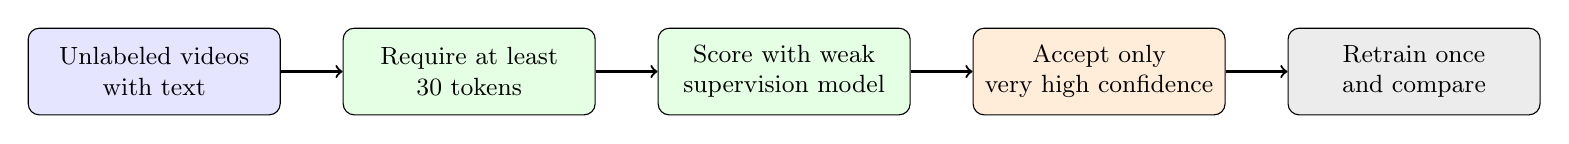
\begin{tikzpicture}[
    box/.style={draw, rounded corners, align=center, minimum width=3.2cm, minimum height=1.1cm, font=\small},
    arrow/.style={->, thick}
]
\node[box, fill=blue!10] at (0,0) (pool) {Unlabeled videos\\with text};
\node[box, fill=green!10] at (4.0,0) (tokens) {Require at least\\30 tokens};
\node[box, fill=green!10] at (8.0,0) (score) {Score with weak\\supervision model};
\node[box, fill=orange!15] at (12.0,0) (accept) {Accept only\\very high confidence};
\node[box, fill=gray!15] at (16.0,0) (retrain) {Retrain once\\and compare};

\draw[arrow] (pool) -- (tokens);
\draw[arrow] (tokens) -- (score);
\draw[arrow] (score) -- (accept);
\draw[arrow] (accept) -- (retrain);
\end{tikzpicture}
}
\caption{Pseudo-labeling funnel used for the unlabeled pool.}
\label{fig:implementation-pseudo-label-funnel}
\end{figure}

\subsubsection{Final Model Selection}

The final model is selected using validation behavior, not test-set tuning. Pseudo-labeling is kept only if it does not reduce validation macro-F1 or harmful-class recall compared with the weak-supervision model. The selected augmented model is then compared with the expert-only baseline.

\begin{verbatim}
if pseudo_macro_f1 >= weak_macro_f1
   and pseudo_recall >= weak_recall:
    selected_augmented_model = pseudo_model
else:
    selected_augmented_model = weak_model
\end{verbatim}

This rule makes pseudo-labeling an empirical question. If it helps, it can be selected; if it hurts validation performance, it is reported as a negative result and not shipped.

\subsubsection{Demo Prediction API}

After model selection, the final classifier is exposed through a small local API. The prediction request contains title, description, and transcript fields, with at least one required. The response contains:

\begin{itemize}
    \item \textbf{is\_harmful}: binary harmful decision.
    \item \textbf{harmful\_probability}: calibrated harmful probability.
    \item \textbf{risk\_band}: low, medium, or high.
    \item \textbf{model\_version}: selected model version.
\end{itemize}

The risk band is computed as:

\begin{verbatim}
if probability < 0.35:
    risk_band = "low"
elif probability <= 0.65:
    risk_band = "medium"
else:
    risk_band = "high"
\end{verbatim}

The API is intended as a demonstration interface for short text inputs after the model is loaded. It is not a production moderation service.

\subsection{Results}

\subsubsection{Data Quality Summary}

The pipeline successfully produced the expected processed data layers and audit outputs. Table \ref{tab:implementation-data-quality-summary} summarizes the main data quality results.

\begin{table}[H]
\centering
\small
\renewcommand{\arraystretch}{1.25}
\begin{tabular}{|l|r|}
\hline
\textbf{Metric} & \textbf{Value} \\
\hline
Silver row count & 134420 \\
\hline
Dropped row count & 191 \\
\hline
Wide table row count & 59692 \\
\hline
Expert-labeled rows with text & 18349 \\
\hline
Conflict rows excluded & 0 \\
\hline
Duplicate video identifiers collapsed & 19464 \\
\hline
Strict HHH rows & 5901 \\
\hline
Strict NNN rows & 679 \\
\hline
\end{tabular}
\caption{High-level data quality summary after processing.}
\label{tab:implementation-data-quality-summary}
\end{table}

The large number of collapsed duplicate identifiers is expected because the same videos can appear across multiple annotation sources. The zero conflict count indicates that, after cleanup, no same-annotator harmful/harmless contradictions remained in the final training table.

\subsubsection{Source Count Drift}

The local dataset did not exactly match the earlier planned source counts. The implementation treats the local files as authoritative and reports the drift as a data quality finding.

\begin{table}[H]
\centering
\scriptsize
\renewcommand{\arraystretch}{1.2}
\begin{tabularx}{\textwidth}{|>{\raggedright\arraybackslash}X|r|r|r|}
\hline
\textbf{Metric} & \textbf{Plan} & \textbf{Local} & \textbf{Delta} \\
\hline
Full-agreement unique IDs & 5901 & 5901 & 0 \\
\hline
Subset-agreement unique IDs & 13981 & 13980 & -1 \\
\hline
Domain expert harmful unique IDs & 15058 & 15057 & -1 \\
\hline
Domain expert harmless unique IDs & 3296 & 3294 & -2 \\
\hline
GPT harmful unique IDs & 10494 & 10494 & 0 \\
\hline
GPT harmless unique IDs & 7796 & 7794 & -2 \\
\hline
Crowdworker harmful unique IDs & 12623 & 12622 & -1 \\
\hline
Crowdworker harmless unique IDs & 4376 & 4374 & -2 \\
\hline
Unlabeled unique IDs after deduplication & 59925 & 59671 & -254 \\
\hline
\end{tabularx}
\caption{Reference-count drift between planned values and local authoritative files.}
\label{tab:implementation-count-drift}
\end{table}

Most labeled-source differences are small. The unlabeled pool has a larger deduplication drift, but this does not invalidate the experiment because all training and evaluation steps use the same cleaned local source truth.

\subsubsection{Text Coverage}

Text availability is central because the core model uses only title, description, and transcript. After canonical consolidation, almost every wide-table row contains at least one usable text field.

\begin{table}[H]
\centering
\small
\renewcommand{\arraystretch}{1.25}
\begin{tabular}{|l|r|}
\hline
\textbf{Coverage metric} & \textbf{Count} \\
\hline
Wide rows & 59692 \\
\hline
Rows with any text & 59690 \\
\hline
Rows with title & 59627 \\
\hline
Rows with description & 53640 \\
\hline
Rows with transcript & 43331 \\
\hline
Rows with published date & 59593 \\
\hline
\end{tabular}
\caption{Canonical wide-table text coverage.}
\label{tab:implementation-text-coverage}
\end{table}

The unlabeled pool also has strong text coverage after normalization: all 60904 unlabeled silver rows contain at least one text field, including 60841 titles, 54661 descriptions, and 44134 transcripts. This correction is important because pseudo-labeling depends on text-bearing unlabeled examples.

\subsubsection{Annotator Agreement Results}

Table \ref{tab:implementation-agreement} reports pairwise agreement between domain expert, GPT-4-Turbo, and crowdworker labels.

\begin{table}[H]
\centering
\small
\renewcommand{\arraystretch}{1.25}
\begin{tabular}{|l|r|r|r|}
\hline
\textbf{Pair} & \textbf{Overlap} & \textbf{Agreement} & \textbf{Kappa} \\
\hline
Domain expert vs GPT-4-Turbo & 17514 & 0.6606 & 0.2485 \\
\hline
Domain expert vs crowdworker & 16143 & 0.6597 & 0.0331 \\
\hline
GPT-4-Turbo vs crowdworker & 16087 & 0.5527 & 0.0630 \\
\hline
\end{tabular}
\caption{Pairwise annotator agreement on overlapping videos.}
\label{tab:implementation-agreement}
\end{table}

\begin{figure}[H]
\centering
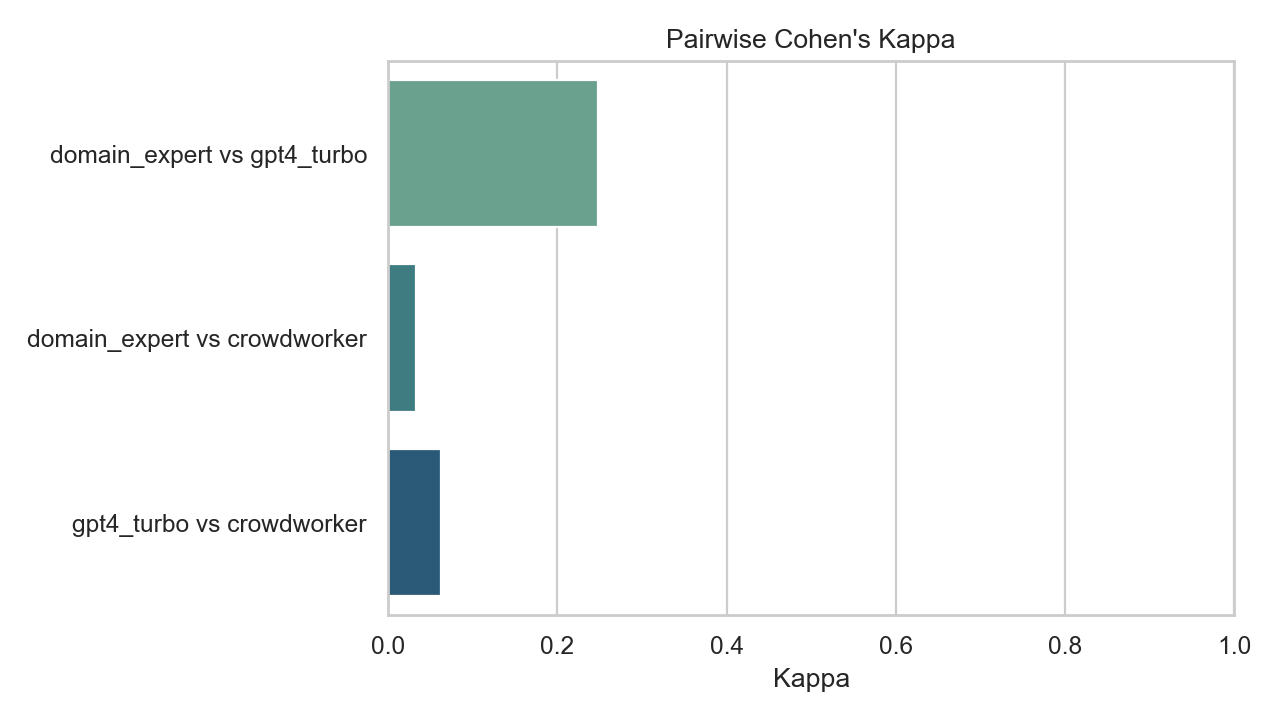
\includegraphics[width=0.82\textwidth]{uploads/implementation_agreement_kappa.png}
\caption{Pairwise Cohen's kappa for the three binary label sources.}
\label{fig:implementation-agreement-kappa}
\end{figure}

The kappa values show that the weak sources are noisy relative to domain experts. GPT-4-Turbo has stronger chance-adjusted agreement with domain expert labels than crowdworkers, but neither weak source is reliable enough to be treated as ground truth. This supports the decision to use weighted weak supervision with abstention.

\subsubsection{Weak-Supervision Results}

The weak-supervision step estimated nearly equal normalized reliability weights for the two weak sources:

\begin{itemize}
    \item GPT-4-Turbo weight: 0.499106.
    \item Crowdworker weight: 0.500894.
\end{itemize}

The weak-label acceptance summary is shown in Table \ref{tab:implementation-weak-labels}.

\begin{table}[H]
\centering
\small
\renewcommand{\arraystretch}{1.25}
\begin{tabular}{|l|r|}
\hline
\textbf{Weak-label metric} & \textbf{Value} \\
\hline
Candidate rows & 940 \\
\hline
Accepted rows & 648 \\
\hline
Accepted harmful rows & 493 \\
\hline
Accepted harmless rows & 155 \\
\hline
\end{tabular}
\caption{Weak-label acceptance summary.}
\label{tab:implementation-weak-labels}
\end{table}

Weak supervision adds a modest number of additional training rows. Because the accepted rows are restricted by confidence and leakage rules, the augmentation is conservative rather than simply merging all GPT and crowdworker labels.

\subsubsection{Pseudo-Labeling Results}

Pseudo-labeling was exercised on the corrected unlabeled pool. Table \ref{tab:implementation-pseudo-labels} shows the acceptance funnel.

\begin{table}[H]
\centering
\small
\renewcommand{\arraystretch}{1.25}
\begin{tabular}{|l|r|}
\hline
\textbf{Pseudo-label funnel metric} & \textbf{Value} \\
\hline
Rows with any text & 40401 \\
\hline
Rows after holdout exclusion & 40401 \\
\hline
Rows with at least 30 tokens & 35676 \\
\hline
Accepted pseudo-labels & 9254 \\
\hline
Accepted harmful pseudo-labels & 9253 \\
\hline
Accepted harmless pseudo-labels & 1 \\
\hline
Kept for final model & No \\
\hline
\end{tabular}
\caption{Pseudo-label acceptance funnel.}
\label{tab:implementation-pseudo-labels}
\end{table}

Although many pseudo-labels were accepted, they were almost entirely harmful. The pseudo-label model reduced validation macro-F1 compared with the weak-supervision model, so it was not selected as the final model. This is an important negative result: larger training data did not automatically produce a better classifier.

\subsubsection{Model Comparison}

The main binary test results are shown in Table \ref{tab:implementation-model-comparison}. All trained models beat the majority baseline on macro-F1. The weak-supervision model gives the best test macro-F1 among the three trained variants, while pseudo-labeling reduces macro-F1.

\begin{table}[H]
\centering
\scriptsize
\renewcommand{\arraystretch}{1.25}
\begin{tabularx}{\textwidth}{|>{\raggedright\arraybackslash}X|r|r|r|r|r|r|}
\hline
\textbf{Model} & \textbf{Macro-F1} & \textbf{Weighted F1} & \textbf{Precision} & \textbf{Recall} & \textbf{AUROC} & \textbf{PR-AUC} \\
\hline
Majority baseline & 0.4507 & 0.7397 & 0.8206 & 1.0000 & 0.5000 & 0.8206 \\
\hline
Expert only & 0.5701 & 0.7821 & 0.8400 & 0.9712 & 0.7442 & 0.9267 \\
\hline
Expert + weak supervision & 0.5740 & 0.7842 & 0.8408 & 0.9726 & 0.7443 & 0.9274 \\
\hline
Expert + weak supervision + pseudo-labeling & 0.5665 & 0.7809 & 0.8392 & 0.9726 & 0.7411 & 0.9276 \\
\hline
\end{tabularx}
\caption{Expert test split metrics for the majority baseline and trained model variants.}
\label{tab:implementation-model-comparison}
\end{table}

\begin{figure}[H]
\centering
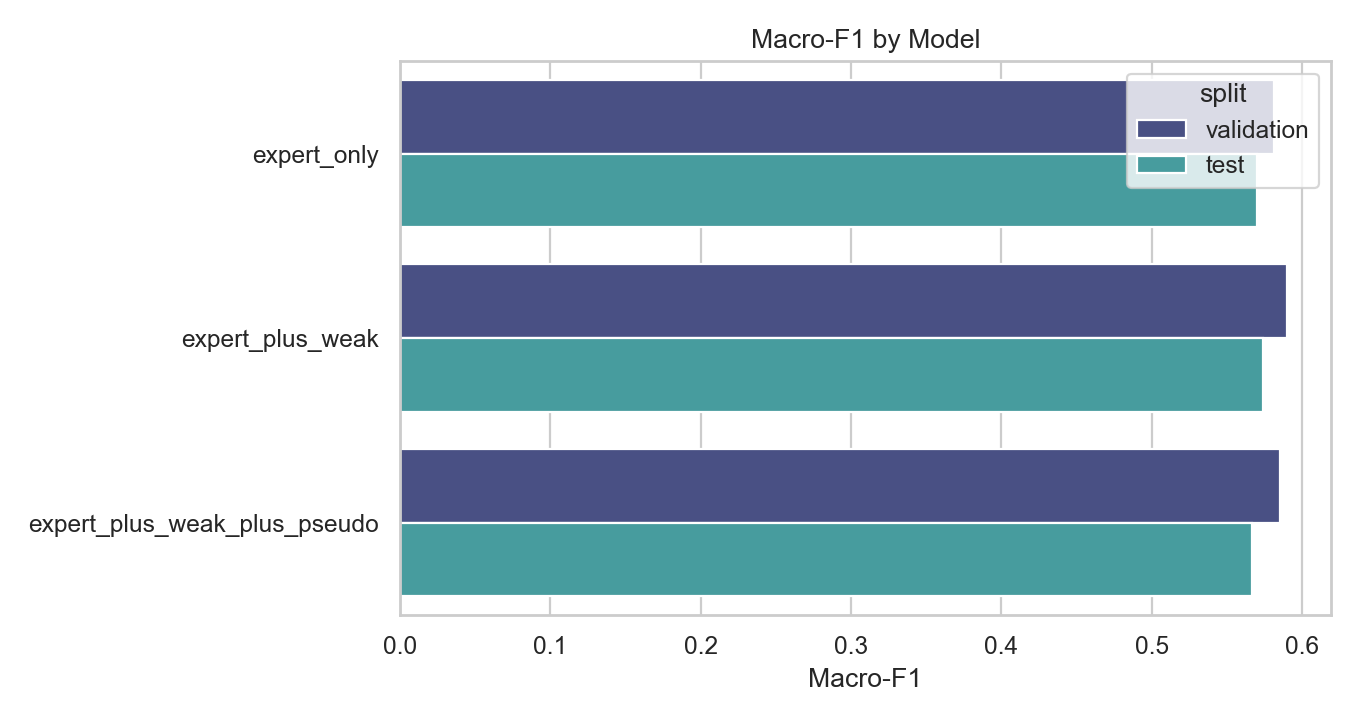
\includegraphics[width=0.82\textwidth]{uploads/implementation_model_macro_f1.png}
\caption{Macro-F1 comparison across trained model variants and data splits.}
\label{fig:implementation-model-macro-f1}
\end{figure}

The final selected model is the expert plus weak-supervision model. It improves expert test macro-F1 from 0.5701 to 0.5740 and slightly improves recall from 0.9712 to 0.9726. The improvement is modest, but it is consistent with the validation-based selection rule.

\subsubsection{Confusion Matrix Analysis}

The confusion matrices in Table \ref{tab:implementation-confusion-matrices} show the main error tradeoff. The final weak-supervision model reduces false negatives from 65 to 62 compared with the expert-only baseline and slightly increases true negatives from 76 to 78.

\begin{table}[H]
\centering
\small
\renewcommand{\arraystretch}{1.25}
\begin{tabular}{|l|r|r|r|r|}
\hline
\textbf{Model} & \textbf{TN} & \textbf{FP} & \textbf{FN} & \textbf{TP} \\
\hline
Expert only & 76 & 418 & 65 & 2194 \\
\hline
Expert + weak supervision & 78 & 416 & 62 & 2197 \\
\hline
Expert + weak supervision + pseudo-labeling & 73 & 421 & 62 & 2197 \\
\hline
\end{tabular}
\caption{Expert test split confusion matrices, flattened as TN, FP, FN, and TP.}
\label{tab:implementation-confusion-matrices}
\end{table}

The model achieves very high harmful-class recall, which is useful for moderation triage. However, the number of false positives remains high. This explains why macro-F1 is much lower than harmful-class recall and shows that threshold selection matters for practical use.

\subsubsection{Validation Threshold Sweep}

The default binary decision threshold is 0.5, but a threshold sweep was performed on the validation split to understand the precision-recall tradeoff. Table \ref{tab:implementation-threshold-sweep} reports the best validation thresholds by macro-F1.

\begin{table}[H]
\centering
\small
\renewcommand{\arraystretch}{1.25}
\begin{tabular}{|l|r|r|r|r|}
\hline
\textbf{Model} & \textbf{Threshold} & \textbf{Macro-F1} & \textbf{Precision} & \textbf{Recall} \\
\hline
Expert only & 0.70 & 0.6619 & 0.8771 & 0.8853 \\
\hline
Expert + weak supervision & 0.70 & 0.6605 & 0.8769 & 0.8835 \\
\hline
Expert + weak supervision + pseudo-labeling & 0.75 & 0.6574 & 0.8898 & 0.8264 \\
\hline
\end{tabular}
\caption{Best validation thresholds by macro-F1 for the trained model variants.}
\label{tab:implementation-threshold-sweep}
\end{table}

The threshold sweep shows that higher thresholds can improve macro-F1 by reducing false positives, but they also reduce harmful-class recall. A real moderation workflow could choose a threshold based on review capacity and the relative cost of false positives and false negatives.

\subsubsection{Strict Consensus Benchmark}

The strict consensus benchmark evaluates videos where all three label sources agree: \texttt{HHH} for harmful and \texttt{NNN} for harmless. This benchmark is expected to be easier because it focuses on less ambiguous examples.

\begin{table}[H]
\centering
\scriptsize
\renewcommand{\arraystretch}{1.25}
\begin{tabularx}{\textwidth}{|>{\raggedright\arraybackslash}X|r|r|r|r|r|r|}
\hline
\textbf{Model} & \textbf{Macro-F1} & \textbf{Weighted F1} & \textbf{Precision} & \textbf{Recall} & \textbf{AUROC} & \textbf{PR-AUC} \\
\hline
Expert only & 0.6732 & 0.8995 & 0.9254 & 0.9867 & 0.8597 & 0.9803 \\
\hline
Expert + weak supervision & 0.6845 & 0.9035 & 0.9266 & 0.9901 & 0.8647 & 0.9809 \\
\hline
Expert + weak supervision + pseudo-labeling & 0.6722 & 0.9002 & 0.9247 & 0.9901 & 0.8583 & 0.9800 \\
\hline
\end{tabularx}
\caption{Strict HHH/NNN consensus benchmark metrics.}
\label{tab:implementation-consensus-benchmark}
\end{table}

The weak-supervision model improves consensus macro-F1 from 0.6732 to 0.6845. This supports the conclusion that weak supervision improves robustness on clearer, high-agreement examples, even though the overall gain is small.

\subsubsection{Error Analysis}

The final model's errors were grouped into correct high-confidence predictions, false positives, false negatives, and missing-transcript cases. Table \ref{tab:implementation-error-examples} shows representative examples.

\begin{table}[H]
\centering
\scriptsize
\renewcommand{\arraystretch}{1.25}
\begin{tabularx}{\textwidth}{|p{2.8cm}|p{2.4cm}|r|r|r|X|}
\hline
\textbf{Case type} & \textbf{Video ID} & \textbf{Prob.} & \textbf{Pred.} & \textbf{True} & \textbf{Title} \\
\hline
Correct high-confidence & \texttt{QA28Ze6HBME} & 0.9967 & 1 & 1 & The MOST Insane Sh** I've EVER Witnessed !!! \\
\hline
False positive & \texttt{ZR5Wx1aTNXU} & 0.9812 & 1 & 0 & James Webb Telescope Discovers NEW 10th Planet Bigger Than Pluto \\
\hline
False negative & \texttt{OutB8gXxbO0} & 0.4951 & 0 & 1 & My Anorexia Recovery: Thinspo \\
\hline
Missing transcript & \texttt{C7lRtA83SQM} & 0.9903 & 1 & 1 & BIG LOST IN CASINO LAS VEGAS ROULETTE HOT BET TABLE HOT EXCLUSIVE 2023-04-08 \\
\hline
\end{tabularx}
\caption{Representative final-model prediction examples from the expert test split.}
\label{tab:implementation-error-examples}
\end{table}

The false positive example suggests that sensational wording can resemble harmful-content language even when the domain expert label is harmless. The false negative example shows the opposite risk: a harmful or sensitive topic may be framed in a recovery-oriented or ambiguous way, making the text signal harder to classify. Missing or noisy transcripts remain a key limitation for a text-first system.

\subsubsection{Demo API Verification}

The local demo API was verified against three practical requirements: empty inputs are rejected, repeated identical inputs produce deterministic outputs, and average prediction latency after model load remains under one second. The response format includes the binary harmful decision, harmful probability, risk band, and model version.

\begin{table}[H]
\centering
\small
\renewcommand{\arraystretch}{1.25}
\begin{tabularx}{\textwidth}{|>{\raggedright\arraybackslash}p{4.5cm}|>{\raggedright\arraybackslash}X|}
\hline
\textbf{API behavior} & \textbf{Verification result} \\
\hline
Reject empty title, description, and transcript & Passed \\
\hline
Return required fields in prediction response & Passed \\
\hline
Return deterministic output for repeated identical input & Passed \\
\hline
Average latency below one second after model load & Passed \\
\hline
\end{tabularx}
\caption{Demo API verification summary.}
\label{tab:implementation-api-verification}
\end{table}

This confirms that the final model can be used through a lightweight local interface after the batch training workflow is complete.

\subsubsection{Overall Result}

The final selected model is \texttt{expert\_plus\_weak}. It is selected because weak supervision improves validation and test macro-F1 relative to the expert-only baseline, while pseudo-labeling reduces validation macro-F1 and is therefore rejected by the fallback rule. The final test metrics are:

\begin{itemize}
    \item Macro-F1: 0.5740.
    \item Weighted F1: 0.7842.
    \item Precision: 0.8408.
    \item Recall: 0.9726.
    \item AUROC: 0.7443.
    \item PR-AUC: 0.9274.
\end{itemize}

The main conclusion is that the implemented pipeline successfully builds reproducible data layers, performs auditable label consolidation, compares supervised and weakly supervised models fairly, exercises pseudo-labeling, and exposes the selected binary classifier through a local API. Weak supervision provides a modest improvement, while pseudo-labeling is documented as a negative result under the validation-based selection rule.
